\chapter{基于多维度特征的PE识别结果与分析}
\section{引言}
\section{模型评估指标}
\subsection{性能度量方法}
一、混淆矩阵

混淆矩阵(confusion matrix)是评估分类器分类效果优劣的常用工具\cite{Zhou2016,Aurélien2018}。其总体思路就是分别统计A类别实例被划分成B类别实例的数目。理论上混淆矩阵的行列没有上限,而在实际应用中,二分类任务的混淆矩阵是最常见的。
此时,将样例依据其真实所属类别与分类器预测类别进行组合可得到四种结果:真阳性(true positive,TP)、假阳性(false positive,FP)、真阴性(true negative,TN)及假阴性(false negative,TN),如\autoref{tab:cm}所示。此时显然有
$TP+FP+TN+FN=\text{样例总数}$。
\begin{table}[htbp]
      \centering
      \caption{\label{tab:cm}二分类任务的混淆矩阵}
      \begin{tabular}{ccc}
      \toprule
      \multicolumn{1}{c}{\multirow{2}[4]{*}{\textbf{真实情况}}} & \multicolumn{2}{c}{\textbf{预测结果}} \\
            \cmidrule{2-3}          & 阳性(1) & 阴性(0) \\
      \midrule
      阳性(1) & 真阳性(TP) & 假阴性(FN) \\
      阴性(0) & 假阳性(FP) & 真阴性(TN) \\
      \bottomrule
      \end{tabular}%
\end{table}%

为量化分类器的具体性能,人们在混淆矩阵的基础上衍生定义了一系列数字指标,包括查全率(recall)、查准率(precison)、准确率(accuracy)及特异性(specificity)等,如\autoref{equ:measures}所示。
\begin{equation}
      \label{equ:measures}
      \left \{
      \begin{aligned}
            Recall      &=\frac{TP}{TP+FN}         \\
            Precison    &=\frac{TP}{TP+FP}          \\
            Accuracy    &=\frac{TP+TN}{TP+FP+TN+FN} \\
            Specificity &=\frac{TN}{TN+FP}       \\
      \end{aligned}
      \right.
\end{equation}
其中,查全率亦称召回率、灵敏性(sensitivity)或真阳性率(true positive rate,TPR),查准率亦称精准率,特异性亦称真阴性率。查全率与查准率是应用的最广泛的两个指标\cite{Zhou2016,Aurélien2018}。
一般而言,查全率与查准率是对相互矛盾的度量指标,一个指标性能的提高意味着另一个指标性能的下降。通常只有在简单分类任务中,
才能同时获得较高的查准率与查全率。这称为精度-召回率权衡。为评估查全率与查准率均不相等的分类器性能,人们进一步定义了$F_1\text{分数}$,如\autoref{equ:f1}所示。
\begin{equation}
      \label{equ:f1}
      F_1=\frac{2}{\frac{1}{Precison}+\frac{1}{Recall}}=\frac{2\cdot Precison\cdot Recall}{Precison+Recall}=\frac{TP}{TP+\frac{FN+FP}{2}}
\end{equation}
$F_1\text{分数}$是召回率与精准率的谐波均值。召回率与精准率相近的分类器易获得更高的$F_1\text{分数}$。

在评估分类器性能时需要根据场景,从\autoref{equ:measures}与\autoref{equ:f1}中灵活选取恰当的评价指标。

二、ROC曲线、AUC与约登指数

受试者工作特征(Receiver Operating Characteristic,ROC)曲线是另一种常用于二分类问题的分析工具。ROC绘制的是真阳性率和假阳性率(false positive rate,FPR)之间的变化关系,其中
\begin{equation}
      \label{equ:fpr}
      FPR=\frac{TN}{TN+FP}=1-Specificity
\end{equation}
因此,ROC曲线也被称为灵敏度与1-特异性曲线。绘制曲线时,以分类器的预测结果对样例进行升序排列,依次将样本作为阳性进行预测,计算对应的TPR与FPR后,可得一坐标点$({FPR}_i,{TPR}_i)$,最后将所有坐标点连线即可,如\autoref{fig:roc}所示。
其中,虚线表示纯随机分类器的ROC曲线,理想性能的分类器应无限逼近左上角,即坐标点$(0,1)$。
\begin{figure}[htbp]
      \centering
      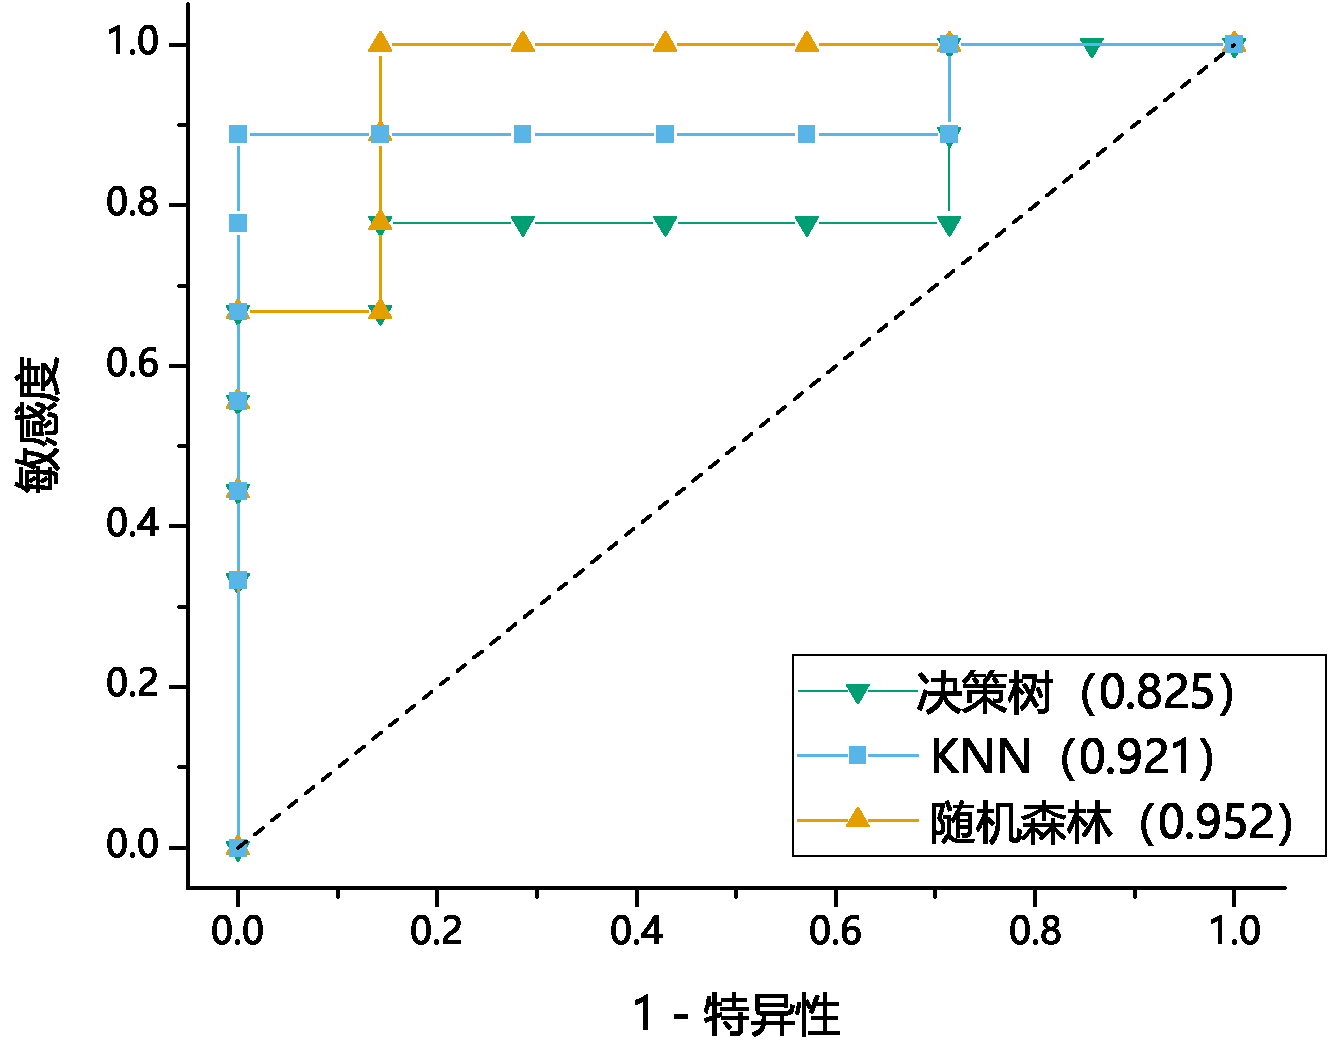
\includegraphics[width=.6\linewidth]{data_plan/roc}
      \caption[ROC曲线与AUC数值]{\label{fig:roc}ROC曲线与AUC数值。各分类器的AUC具体数值参见图例。}
\end{figure}

在衡量多个分类器性能优劣时,常将分类器对应的ROC曲线下面积作为判据,即为AUC(Area Under Curve)。纯随机分类器ROC的AUC数值为0.5,而理想分类器ROC的AUC数值为1,如\autoref{fig:roc}所示。

此外,约登指数(Youden Index)也是用来评价分类器效果的一个指标。若在评估分类器性能时,给予将分类器假阴性和假阳性以相同权重,即可应用约登指数
\begin{equation}
      \label{equ:yi}
      \begin{aligned}
            YI&=Sensitivity-(1-Specificity)\\
            &=Sensitivity+Specificity-1
      \end{aligned}
\end{equation}
一般认为,当YI取值最大时,此时对应的分类阈值为最佳阈值\cite{cwl}。
\section{具体模型表现对比}

\section{聚类分析}
聚类分析是无监督学习的一种,旨在发现数据间是否有潜在的相似性\cite{Liu2018,Li2017}。
因此,我们做了额外的探究——在不给定脉搏波对应的子痫前期的数据标签的基础上,探究能否有效的将数据分成两类,并考察验证分类的效果。

本文进行了以下探究:
1.	分别使用基于ppg 特征的$ppg_feature$ 数据与基于ppg波形数据的$ppg_points $数据,使用sklearn的kmeans 方法进行了聚类分析,其中超参数$n_clusters$被设置为2。
此时,此时若我们将聚类结果作为其学习的分类结果,与数据对应的数据标签进行对照,也可以得到混淆矩阵分别如下

之所以每种分析会得到两个混淆矩阵,是因为聚类分析的簇是不带标签的。两个混淆矩阵是给予簇不同的标签(健康或子痫)。为分析方便,我们选取准确率高的一种聚类结果,即上表中的2、3。并在此基础上进行后续分析。

2.	从表格中可以看到两种数据的聚类分析的准确率分别达到了61.6\%与51.5\%。
基于特征的聚类效果优于直接使用脉搏波波形数据的。
其次,乍一看,数据分类效果并不太好。特别是后者的准确率堪堪超过50\%(典型的随机分类的效果)
但是,我们需要注意到聚类分析的本质是根据数据特征的相似度,也即数据波形的相似度。
因此,让我们来考察下划分出来的波形究竟如何。
于是,我们把图画出来。

此外,我们还需要注意到另外一个变量因素,在PE的影响下,所有患病孕妇的数据波形是会受到影响的,而与正常波形形态有异。因此,所有PE患者都受到了一定程序的医学干预(包括不限于降血压等治疗),目的是使PE患者能够恢复正常水平。因此,会出现假阴性远高于假阳性的现象。可以总结为,在PE确实能改变孕妇脉搏波波形的前提下,聚类分析中出现的假阴性高于假阳性证明是医学干预的必然结果。分析数据与理论分析保持一致。
3.	到具体波形

\begin{figure}[htbp]
    \centering
    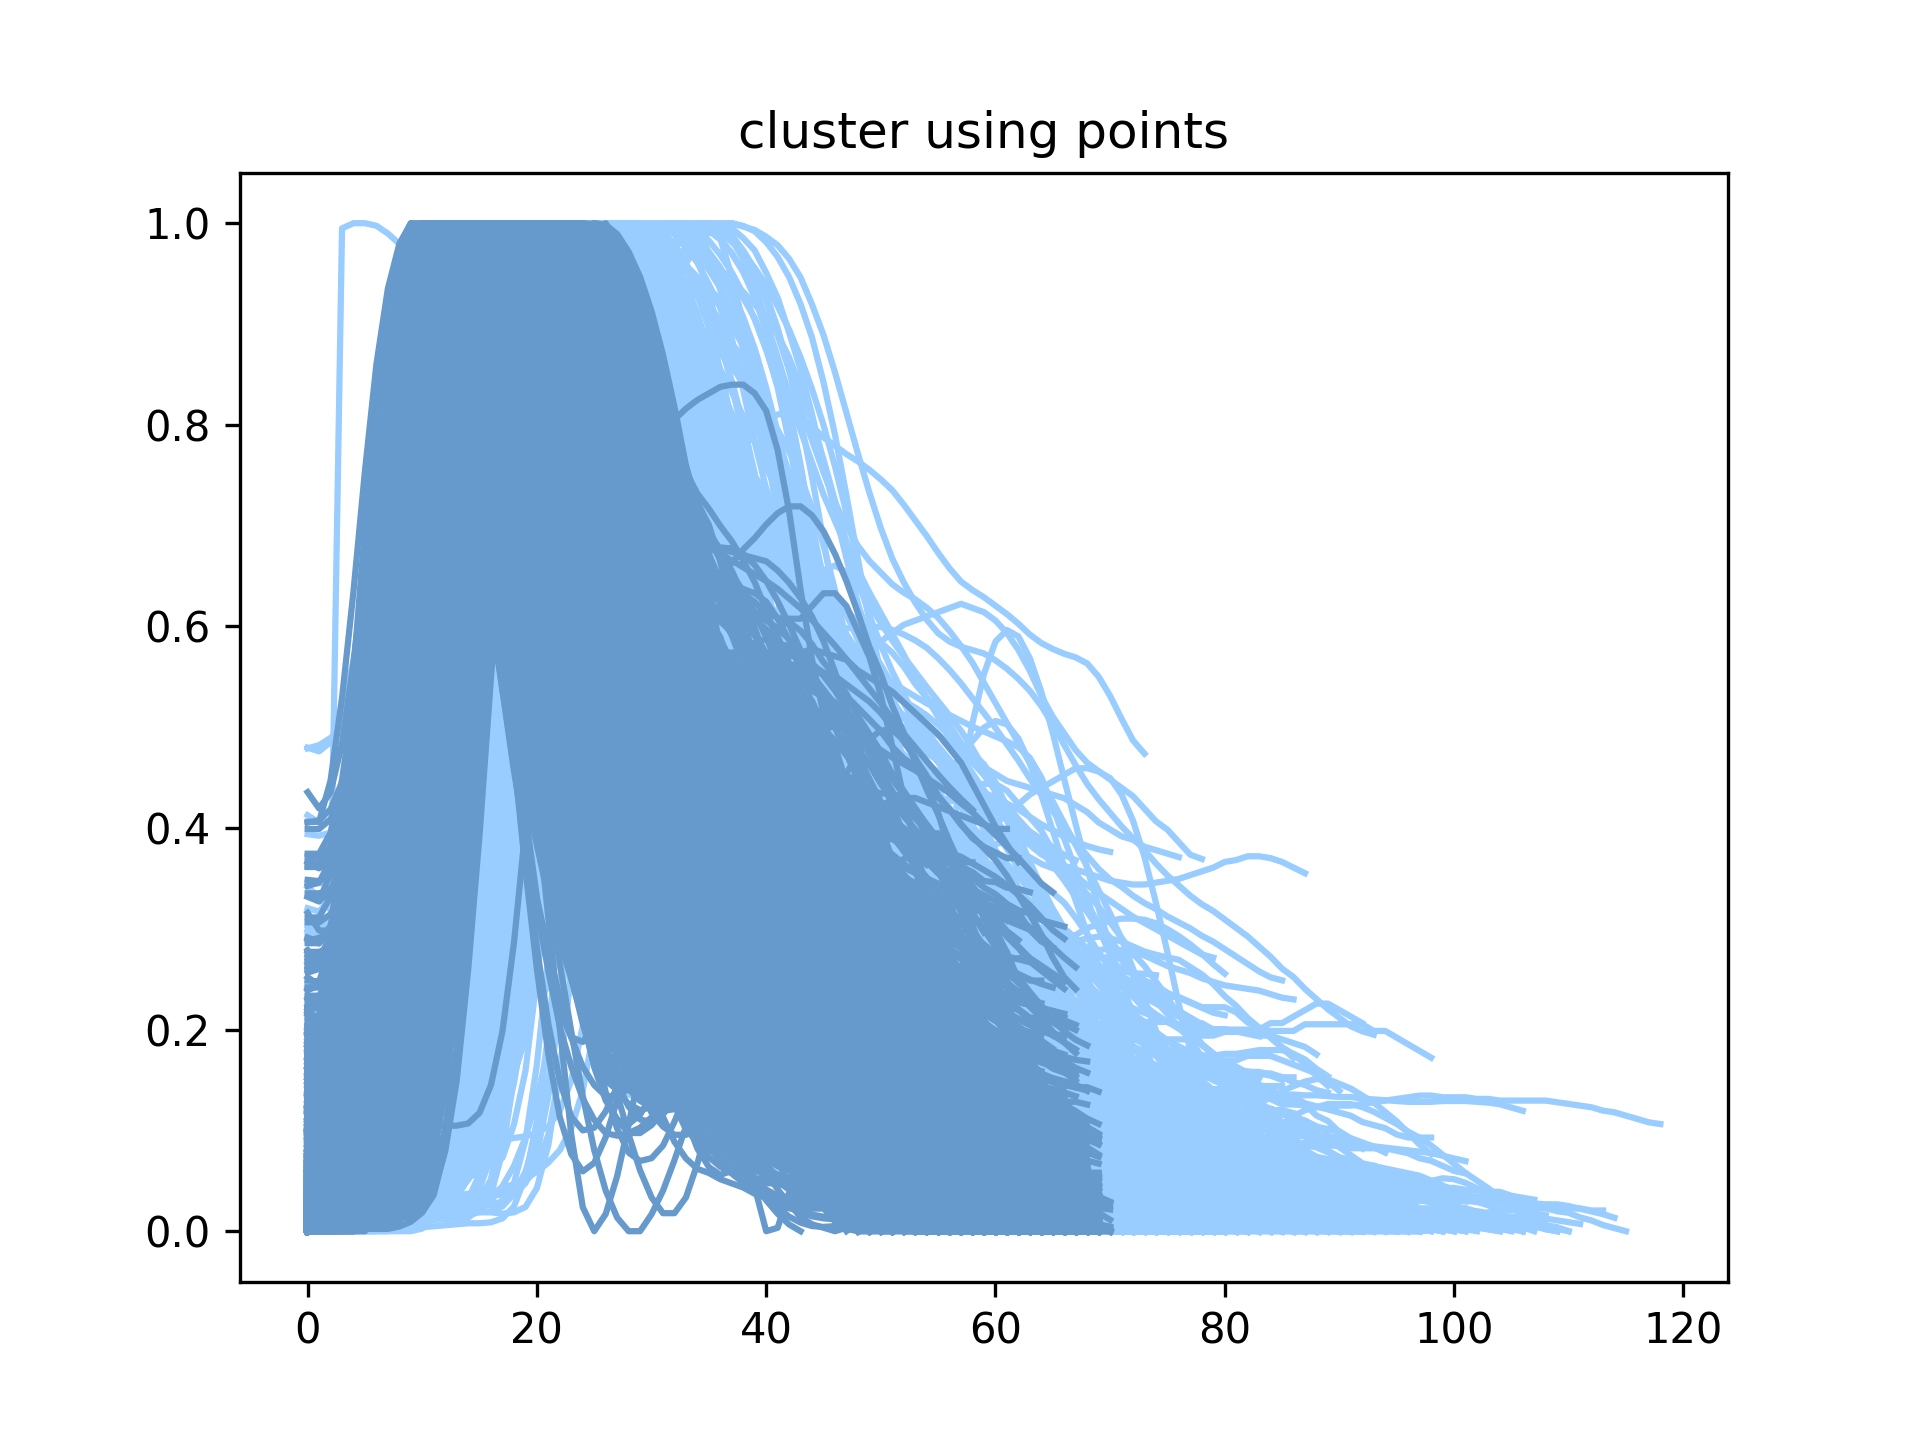
\includegraphics[width=.6\linewidth]{unsupervised/cluster using points_2d}
    \caption[]{\label{fig:cluster2d}111}
\end{figure}
\begin{figure}[htbp]
    \centering
    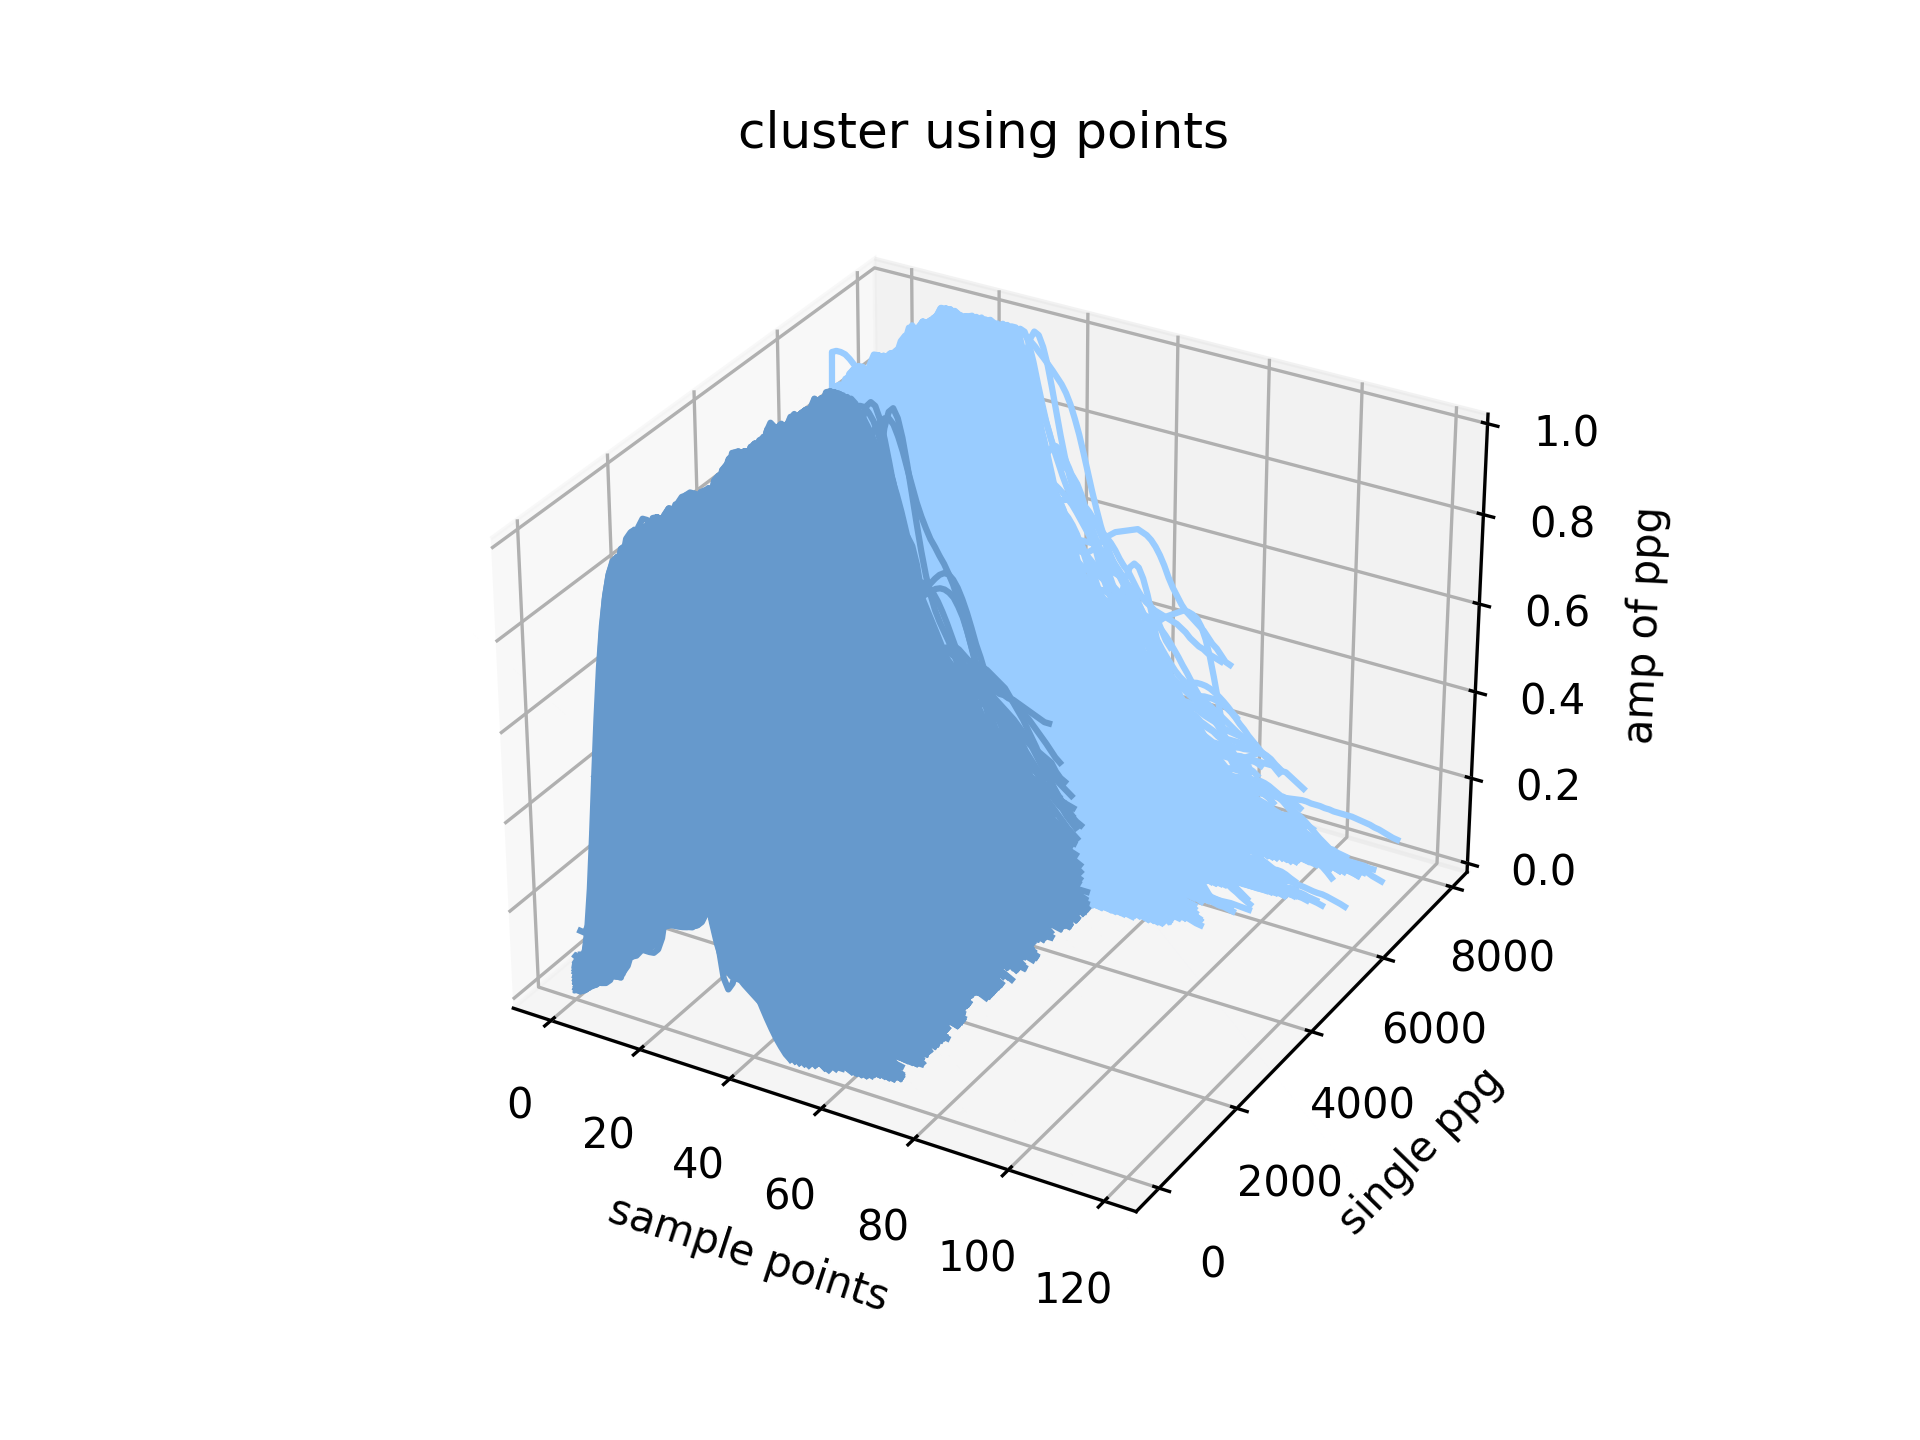
\includegraphics[width=.7\linewidth]{unsupervised/cluster using points_3d}
    \caption[]{\label{fig:cluster3d}222}
\end{figure}
\section{对k的调整与探索}
\section{分析与结论}
\section{小结}